 
\subsubsection { Общие принципы и введение в алгоритм}

Поиск с запретами, как и имитация отжига, относится к методам локального поиска: алгоритм удерживает одно текущее решение и на каждом шаге пытается перейти к соседнему решению, отличающемуся от текущего одним небольшим изменением. Принципиальное отличие от имитации отжига — в способе борьбы с локальными оптимумами. Вместо вероятностного принятия ухудшающих ходов поиск с запретами ведёт явную кратковременную память о недавно совершённых изменениях и временно запрещает (заносит в табу-список) возврат к тем состояниям, из которых алгоритм только что вышел. Это позволяет алгоритму намеренно выбирать на каждом шаге наилучший из доступных соседних вариантов, даже если он хуже текущего решения — то есть осознанно двигаться «в гору» по критерию качества, не рискуя при этом немедленно вернуться назад и зациклиться между двумя соседними состояниями. Единственное исключение из запрета — критерий устремления (aspiration criterion): если запрещённый ход всё равно ведёт к лучшему решению, чем самое лучшее из найденных за всё время работы алгоритма, запрет на этот ход снимается, поскольку явная польза от такого хода перевешивает риск зацикливания.
 
Готовая, в данном случае публичная реализация поиска с запретами (репозиторий edgarsmdn/TS, тот же, что первоначально рассматривался для имитации отжига) была отклонена по той же причине, что и dual_annealing: она реализует поиск с запретами для непрерывных задач, где соседство задаётся через сужающийся радиус вокруг текущей точки в пространстве вещественных чисел, а табу-зона — это область вокруг недавно посещённых точек в этом непрерывном пространстве. У задачи расписания нет естественной метрики «расстояния» между двумя расписаниями, а ход — это не «шаг в случайном направлении», а конкретное, дискретное изменение одного занятия. Поэтому был реализован классический комбинаторный вариант поиска с запретами, восходящий к работам Фреда Гловера, с табу-списком, основанным не на расстоянии между решениями, а на запрете повторения конкретных атрибутов изменения.

\subsubsection { Особенности реализации}

На каждой итерации алгоритм генерирует не один, а целый пакет случайных ходов-кандидатов (типичный размер пакета — около двадцати пяти ходов четырёх видов: изменение дня и пары занятия, замена аудитории, замена преподавателя, обмен временными слотами между двумя занятиями) и выбирает среди них наилучший допустимый — допустимый в смысле «не запрещённый табу-списком либо проходящий по критерию устремления». Если весь пакет кандидатов оказался под запретом, выбирается случайный ход без какой-либо дополнительной проверки — это единственный встроенный механизм диверсификации поиска при затяжном застое.

Табу-список устроен не как список запрещённых полных решений (что было бы естественно для непрерывной версии алгоритма, но бессмысленно для дискретной задачи — вероятность повторно попасть ровно в то же самое расписание из миллионов возможных пренебрежимо мала), а как список запрещённых атрибутов изменения: запоминается не «то самое прошлое расписание», а конкретная связка «дисциплина — вид изменения — прежнее значение», и в течение заданного числа итераций запрещается возвращать именно эту дисциплину именно к этому прежнему значению.

\captionof{listing}{Пример запрета: запрет предыдущего слота}
\begin{minted}{python}
tabu_attrs = [(discipline_id, "slot", (old_weekday, old_timeslot))]
\end{minted}

\subsubsection { Метрики}

\paragraph { Оптимизация размера окрестности поиска}

Мы проанализировали влияние размера батча кандидатов на качество и скорость работы алгоритма. Было выявлено, что увеличение параметра neighborhood_size до 50 не приводит к дальнейшему снижению штрафов, создавая избыточную вычислительную нагрузку. Оптимальным компромиссом для рассматриваемых размерностей является значение 25.

\begin{figure}[h]
    \centering
    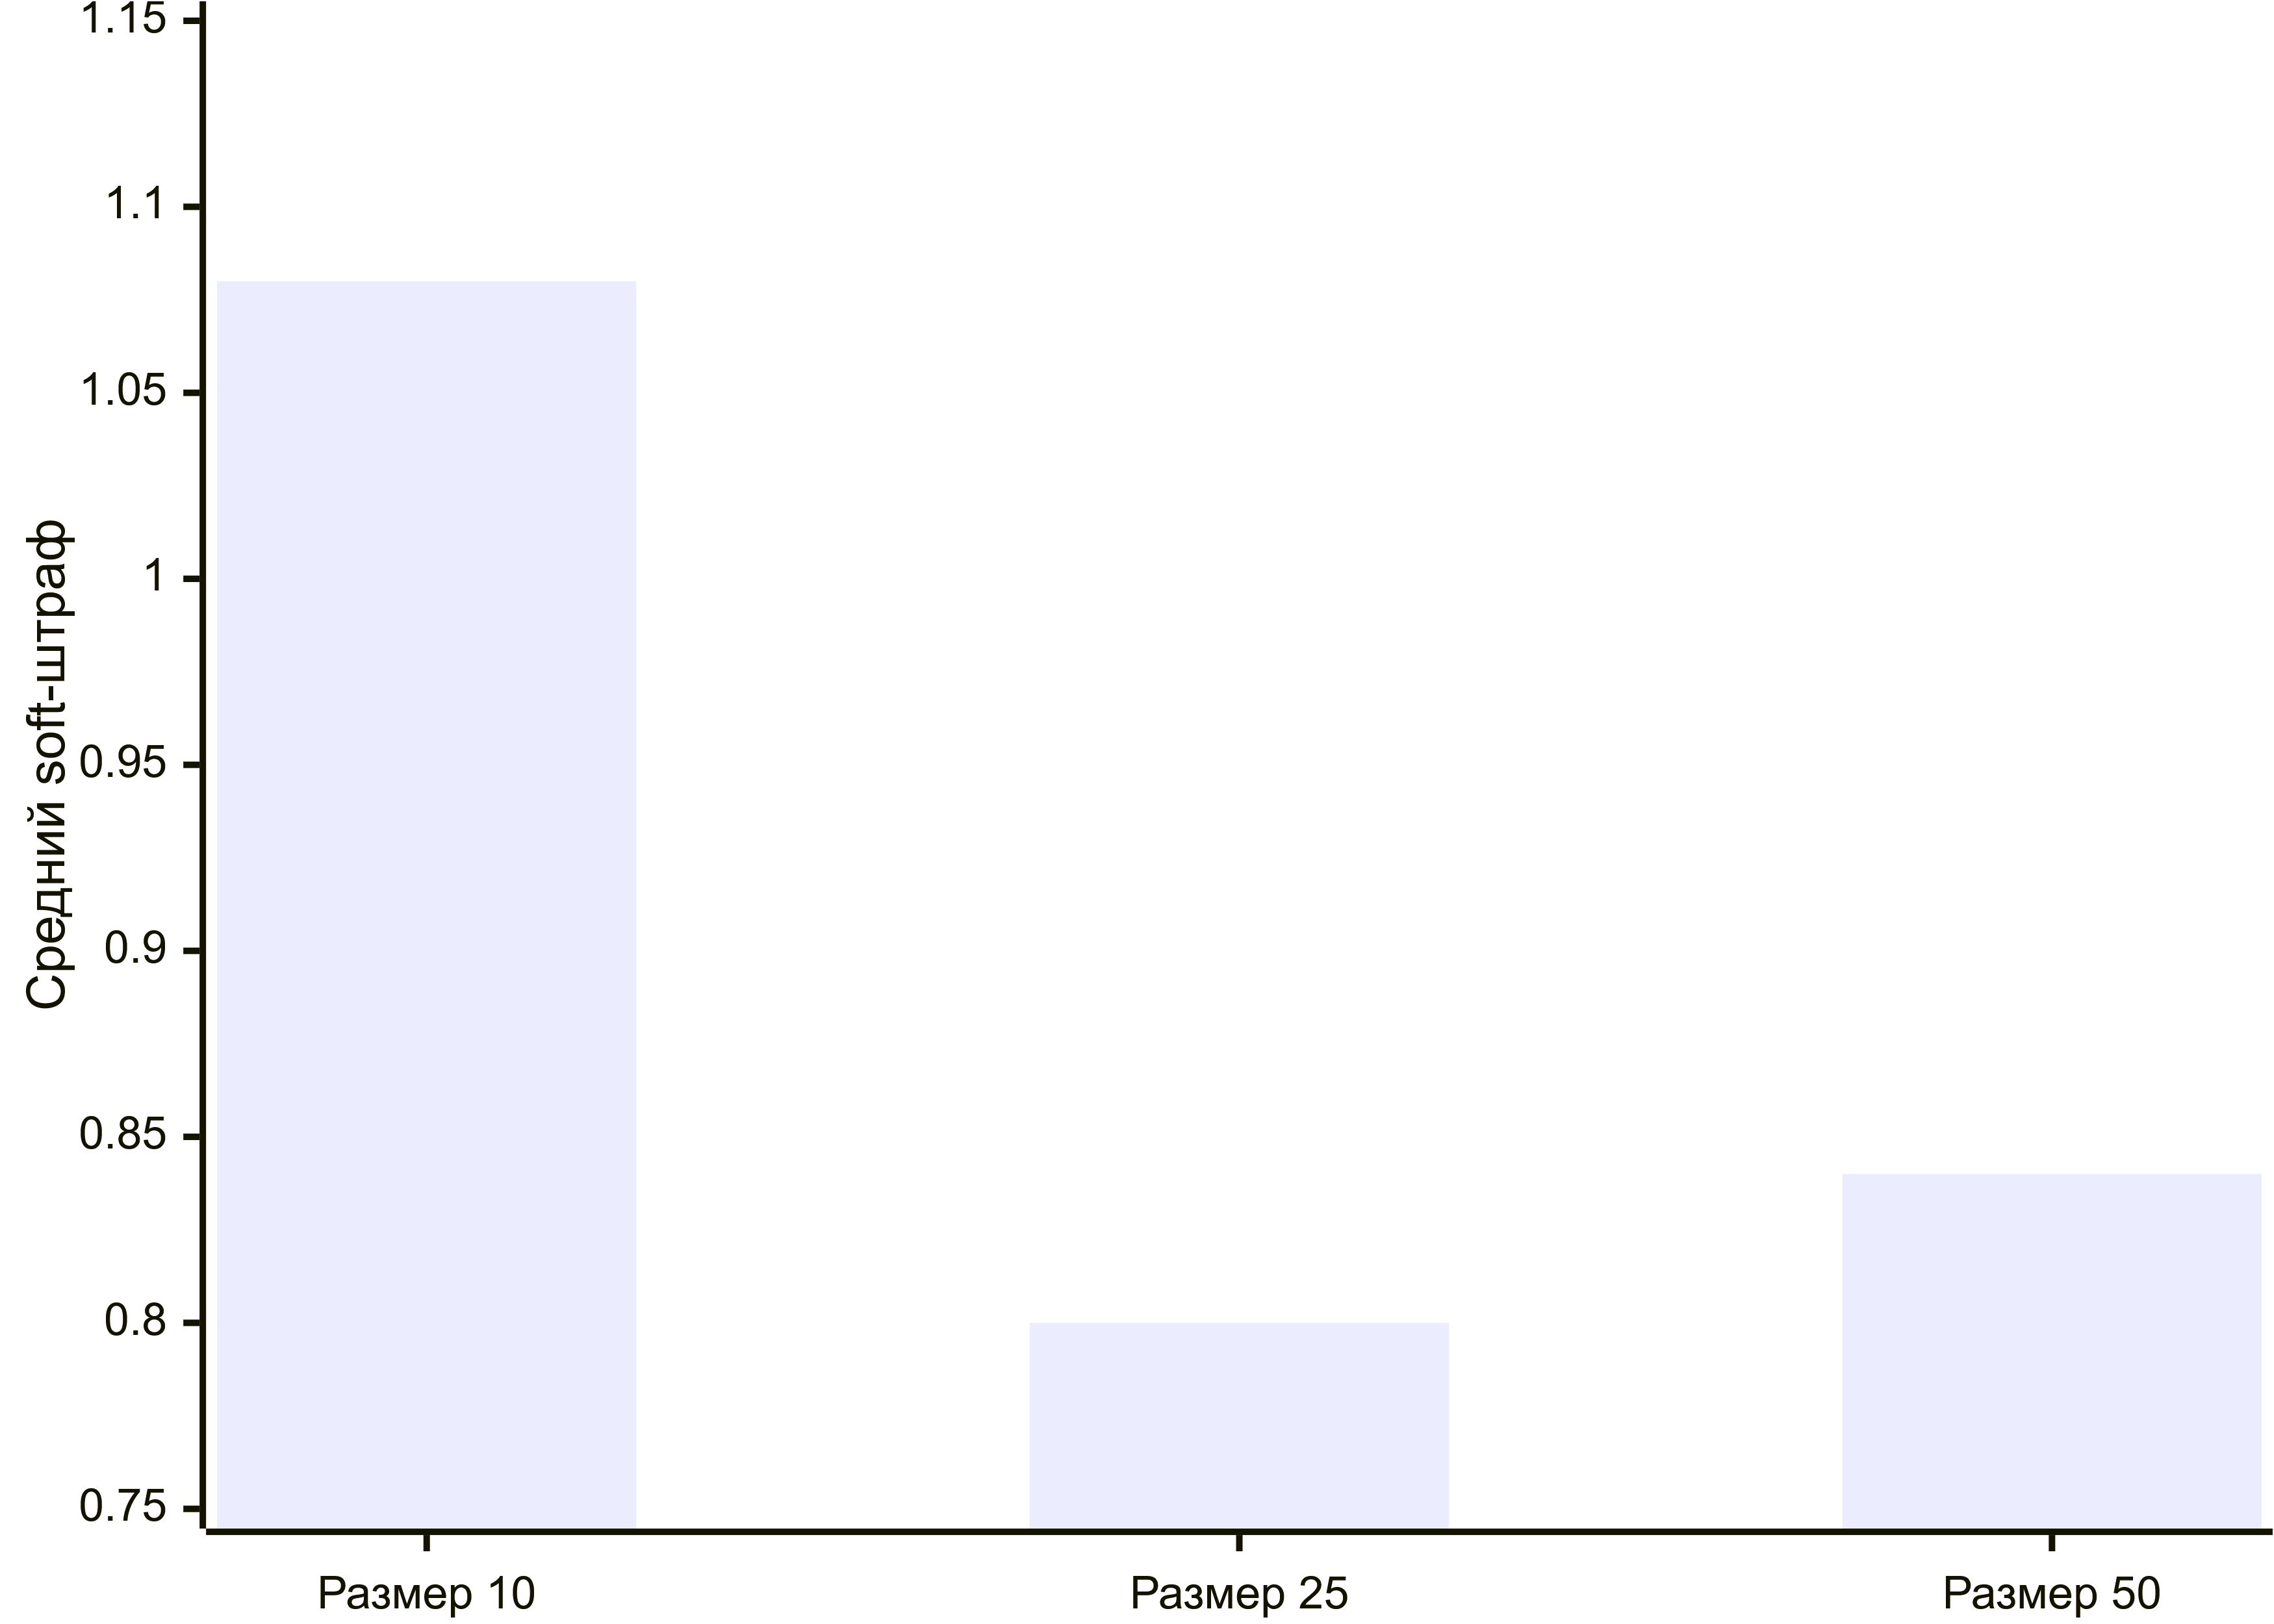
\includegraphics[width=0.8\textwidth]{images/TS neighborhood diff.png}
    \caption{Влияние neighborhood_size на качество решения}
    \label{fig:TSNeighborhoodDiff}
\end{figure}

\paragraph { Динамика поиска}

Процесс сходимости TS носит ступенчатый характер. Выбор лучшего кандидата из окрестности на каждой итерации обеспечивает резкие улучшения целевой функции, которые сменяются периодами стагнации (плато) при достижении локального минимума в рамках текущего региона поиска.

\begin{figure}[h]
    \centering
    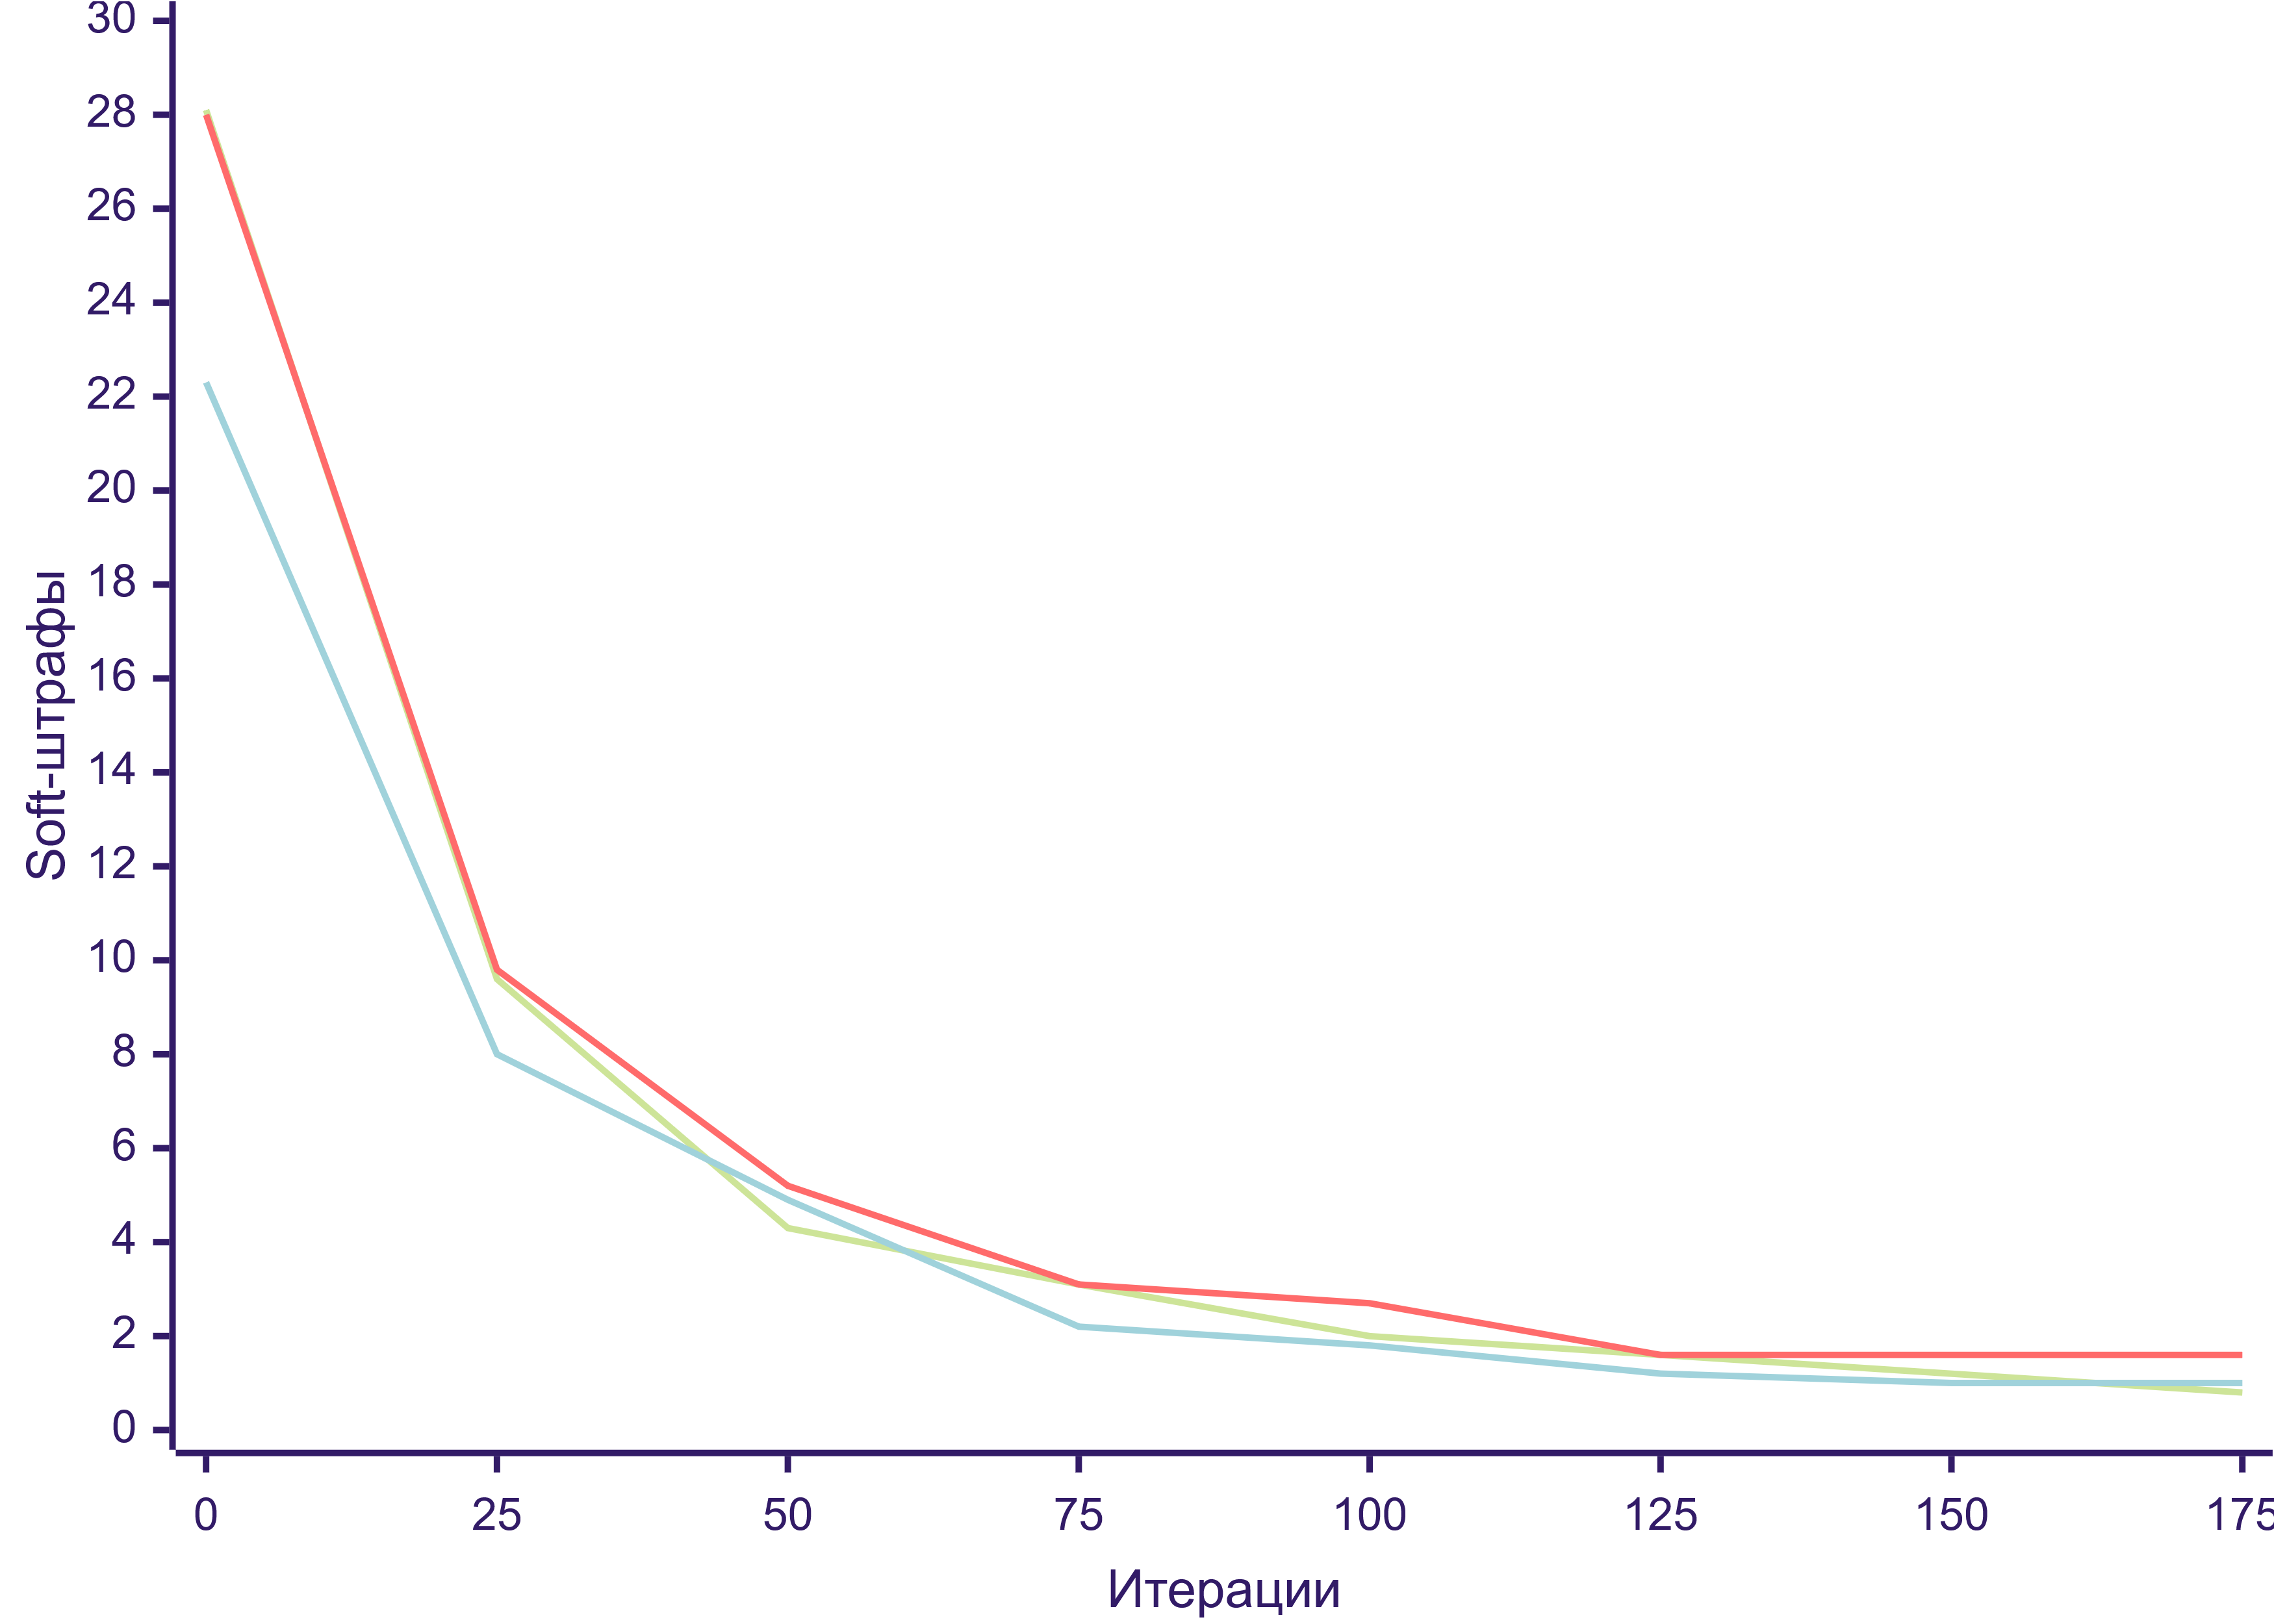
\includegraphics[width=0.8\textwidth]{images/TS Convergence.png}
    \caption{Сходимость TS: динамика soft-штрафов (medium)}
    \label{fig:TSConvergence}
\end{figure}

\subsubsection { Проблемы, возникшие в процессе реализации}

При сопоставлении поиска с запретами с точным методом программирования ограничений (раздел II.4) на крупном наборе данных, заведомо превышающем физическую вместимость учебной сетки, был обнаружен дефект, общий с генетическим алгоритмом и имитацией отжига: контейнер для итогового расписания создавался с ограничением на число занятий, равным вместимости учебной сетки, а не реальному числу занятий в задаче, и лишние занятия незаметно отбрасывались при сборке результата. Особенно показательно, что именно точный метод программирования ограничений — за счёт способности доказывать отсутствие допустимого решения, а не просто сообщать о неудаче поиска — стал той самой опорной точкой, которая позволила опровергнуть ложный вывод о допустимости расписания, построенного поиском с запретами: при заведомой невозможности уместить все занятия в доступные пары точный метод сообщал об отсутствии решения, тогда как поиск с запретами сообщал о найденном допустимом расписании без единого нарушения, что было логическим противоречием, потребовавшим целевой диагностики и приведшим к обнаружению описанного дефекта.

Отдельная архитектурная особенность, выявленная при анализе кода, но не успевшая проявиться в виде наблюдаемой ошибки в рамках проведённого эксперимента, — это потенциальная неоднозначность атрибута табу-запрета в ситуации, когда у одной дисциплины несколько занятий в неделю (например, две лекции). Поскольку запрет привязывается к идентификатору дисциплины, а не к конкретному занятию, теоретически возможна ситуация, при которой запрет, наложенный из-за хода с одним занятием этой дисциплины, ошибочно распространится на другое занятие той же дисциплины, никогда не находившееся в запрещённом состоянии. Это не привело к видимому снижению качества решений в проведённом эксперименте, но обозначено как направление для дальнейшего уточнения реализации.

\subsubsection { Выводы по алгоритму}

Поиск с запретами стабильно показал наилучшее качество решений среди всех четырёх реализованных алгоритмов на всех использованных наборах данных, включая случай, когда задача оказалась структурно неразрешимой и сравнение шло по числу остаточных, неустранимых нарушений. По затраченному времени поиск с запретами оказался медленнее имитации отжига, что объясняется оценкой целого пакета кандидатов на каждой итерации вместо одного хода, но при этом существенно быстрее генетического алгоритма. Сочетание лучшего качества решения с умеренными вычислительными затратами делает поиск с запретами наиболее сбалансированным из четырёх реализованных эвристических методов для рассматриваемой задачи.
